\documentclass{article}
\usepackage{tikz, comment}
\usepackage{pifont}
\usepackage{fontspec}
\usetikzlibrary{arrows, decorations.markings, decorations.pathreplacing}
\begin{comment}
:Title: Not defined yet
:Tags: area using parametric equations,parametric integral formula;average rate of change, arc ;area between curves;area under a curve;arc length of a curve
:Prob: 0.5186;0.3864;0.3777;0.3742;0.3642
:Author: Prof.Hu Ji-shan, HKUST
:Slug: No name yet

Description Here.........
\end{comment}
\begin{document}\centering

\newcommand{\AxisRotator}[1][rotate=0]{%
\tikz [x=0.25cm,y=0.60cm,line width=.2ex,-stealth,#1] \draw (0,0) arc (-165:165:1 and 1);%
}

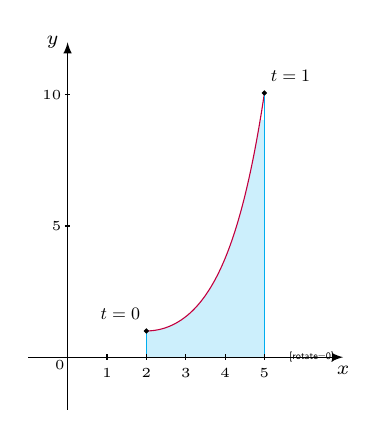
\begin{tikzpicture}[>=latex,xscale=.5*1, yscale=.5/1.5][font=\sf\small]

%\draw[xstep=1cm,ystep=1cm,color=gray!80] (0, -1) grid (8, 8);


\draw[white, fill=cyan!20] ({2+3*(0)}, {0})--++({2+3*(1)-2}, {0})--++({0}, {cosh(3*1)-1})--++({-(2+3*(1)-2)}, {0})--cycle;

\draw[white, fill=white, samples=100, smooth, domain=0:1, variable=\t]
plot ({2+3*(\t)}, {cosh(3*\t)})--({2+3*(0)}, {cosh(3*1)});

\draw[purple, samples=100, smooth, domain=0:1, variable=\t]
plot ({2+3*(\t)}, {cosh(3*\t)});

\draw[cyan] ({2+3*(0)}, {0})--++(0, {cosh(3*0)});
\draw[cyan] ({2+3*(1)}, {0})--++(0, {cosh(3*1)});

\draw[fill, black, xscale=1/1, yscale=1.5] ({2+3*(0)}, {cosh(3*0)/1.5}) circle(0.05)node[left, xshift=0, yshift=6, scale=0.7]{$t=0$};
\draw[fill, black, xscale=1/1, yscale=1.5] ({2+3*(1)}, {cosh(3*1)/1.5}) circle(0.05)node[right, xshift=0, yshift=6, scale=0.7]{$t=1$};

\foreach \x in {1,2,3,4,5}
\draw (\x,2pt*1.5) -- (\x,-2pt*1.5)
node[anchor=north] {\tiny$\x$}
;

\foreach \x in {}
\draw (\x,2pt/2.5) -- (\x,-2pt/2.5)
node[anchor=south] {\tiny$\x$}
;
\foreach \y in {5,10}
\draw (-2pt/1,\y) -- (2pt/1,\y)
node[anchor=east] {\tiny $\y$}
;

\draw[->] (-1, 0) -- (7, 0)node[below] {\scriptsize$x$} node [solid, midway, pos=0.9, scale=0.4]{\AxisRotator[rotate=0]};

\draw[-> ] (0, -2) -- (0, 12)node[left] {\scriptsize$y$} ;

\node[yshift=0] at (-0.2/1, -0.2*1.5) {\tiny$0$};

\end{tikzpicture}
\end{document}